% =============================================================================
\section{Squeezing by component separation}
% =============================================================================

\copypaste{copypaste begins}

\begin{figure}
    %\begin{tabular}{l l}
    %\imagetop{\includegraphics[width=0.85\columnwidth]{riedel_cloud_yz.eps}} & \imagetop{(a)} \\
    %\imagetop{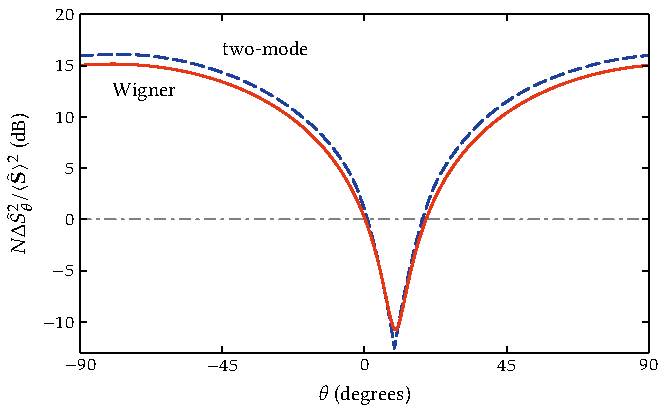
\includegraphics[width=0.85\columnwidth]{riedel_rotation.eps}} & \imagetop{(b)}
    %\end{tabular}

    \caption[]{(color online)
    Reconstructed probability distribution for the value of the spin vector projected on $y,z$ plane (a) and spin noise tomography (b).
    The variance $\Delta^2 \hat{S}_\theta$ is connected to the width of the distribution $d_\theta$ in direction $\theta$
    (blue line between two arrows in panel (a)) as
    $2 \sqrt{\Delta^2 \hat{S}_\theta} = d_\theta$.
    Plot (b) shows the dependence of the normalized variance on the rotation angle $\theta$ for
    the Wigner method (solid red line) and the two-mode variational method (dashed blue line, data taken from~\cite{Riedel2010})
    }
    \label{fig:riedel-rotation}
\end{figure}

The Wigner calculation shows good agreement with other approximate methods like the two-mode variational method~\cite{Li2009} which also includes the effect of particle losses.
As an example consider the recent experiment~\cite{Riedel2010},
where multi-particle entanglement was generated using a state-dependent potential.
A two-component BEC of 1250 atoms was prepared in a cigar-shaped trap with $\omega_x = \omega_y = 2 \pi \times 109\un{Hz}$,
$\omega_z = 2 \pi \times 500\un{Hz}$.
After the first $\pi / 2$-pulse, the potentials for both components were split, leading to the spatial separation of the components.
At $T = 12.7\un{ms}$ they overlapped again, and the second pulse was applied, allowing a measurement of the spin along the angle $\theta$: $\hat{S}_\theta = \hat{S}_z \cos \theta - \hat{S}_y \sin \theta$.
The Wigner method allows us to reconstruct the spin noise distribution in the plane orthogonal to the mean spin (\figref{riedel-rotation}a) and the result can be compared with the two-mode model (\figref{riedel-rotation}b).
Spin tomography shows that the Wigner method predicts about the same shape of spin distribution,
but the values of the maximum squeezing and the maximum unsqueezing are noticeably different than those calculated with the two-mode model.
The calculated value of the quantum noise at maximum squeezing ($-10.73\pm0.05\un{dB}$) is greater than the two-mode model prediction ($-12.8\un{dB}$).
The noise at maximum unsqueezing ($15.16\pm0.05\un{dB}$) is $1\un{dB}$ less than the two-mode model prediction.
We believe this is caused by the Wigner method being a more systematic type of approximation with a small parameter,
and consequently, more suitable for such complex calculations.
Since the technical noise in the experiment reduced the observed squeezing significantly (down to $-3.7\un{dB}$),
more accurate measurements will be necessary to test these differences quantitatively.

\copypaste{copypaste ends}
